\begin{figure} [h]
\centering
         \caption[Zusammenhang Wellenlänge - Wellenzahl]{Dargestellt ist der Zusammenhang zwischen der Wellenlänge $\lambda$ und der Wellenzahl $n$. Da die Phase alle $2\pi$ den gleichen Wert annimmt, wird mit dem Faktor $n$ ein vielfaches der Wellenlänge aufaddiert. Dadurch erhält man die Entfernung zu dem Tag.}
         \label{fig:wavenumber_wavelength}
         \vspace{0.5cm}
         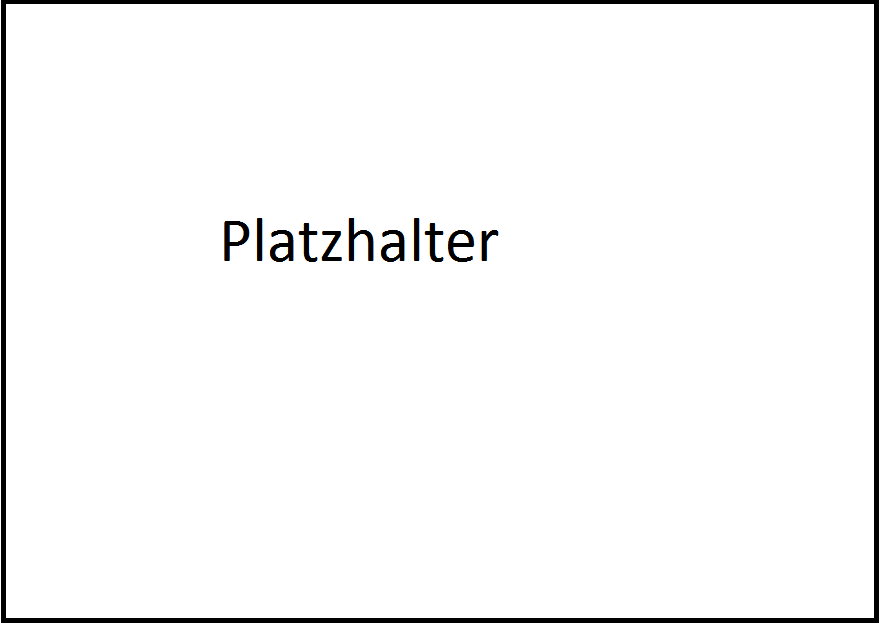
\includegraphics[width=\textwidth]{img/00_placeholder.png}
%      
\end{figure}

Aus der Abbildung~\ref{fig:wavenumber_wavelength} lässt sich folgender Zusammenhang ableiten.
%
\begin{equation}
\label{eq:Phase_Wavenumber}
	d(\Theta, n)=\lambda(\Theta+n)
\end{equation}

\lipsum[1]